\clearpage
\appendix

\section{分组查询注意力中的头组融合}
\label{sec:head-group-fusion}

分组查询注意力（GQA）~\cite{ainslie2023gqa} 允许多个 query 头共享同一组 key-value（KV）头。一个直接实现是为每个 query 头分配独立 GPU threadblock；但当 query 长度较短时，这会使大量潜在 KV-Cache 复用无法被利用。为解决该问题，\sys 提供\emph{头组融合（head-group fusion）}策略：
将不同 KV 头映射到独立 threadblock，同时把 query 头维与 query 长度维进行融合。图~\ref{fig:flashinfer-gqa-packing} 展示了该融合方案中融合后行索引与原始行索引、头索引之间的关系。通过在线程块映射中合并 query-head 维与行维，组内所有 query 头可共享一次 KV-Cache 的共享内存加载，从而提升内存复用与 GQA 吞吐。

\begin{figure}[ht]
    \centering
    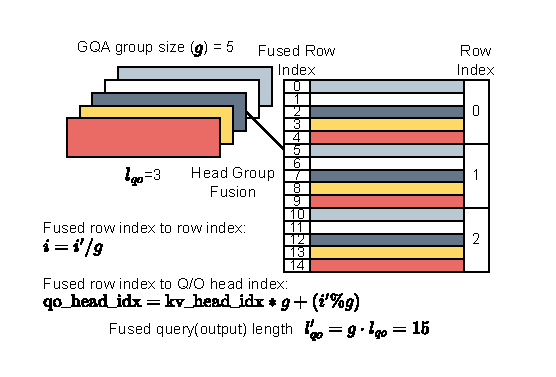
\includegraphics[width=0.5\textwidth]{figures/gqa-mapping.pdf}
    \caption{\sys 在 GQA 中将 query 头与 query 长度维进行头组融合。}
    \label{fig:flashinfer-gqa-packing}
\end{figure}

我们主要在短 query 长度场景下使用头组融合。当 query 长度足够大时，query 维本身已能提供足够工作量来有效利用 KV-Cache，头组融合的重要性会降低。类似思想也在其他框架中出现，例如 TensorRT-LLM~\cite{nvidia2023tensorrt} 中的 XQA~\cite{xqa}。

\section{稀疏 Gather 的开销}
\label{sec:overhead-sparse-gathering}

在第~\ref{sec:sparse-loading} 节中，我们详细介绍了 \sys 的稀疏加载模块：将全局内存中的稀疏行搬运到连续共享内存。本节测量 \sys 在 \emph{decode} 与 \emph{prefill} 两类内核下由稀疏 gather 引入的性能开销。

\begin{figure}[ht]
    \centering
    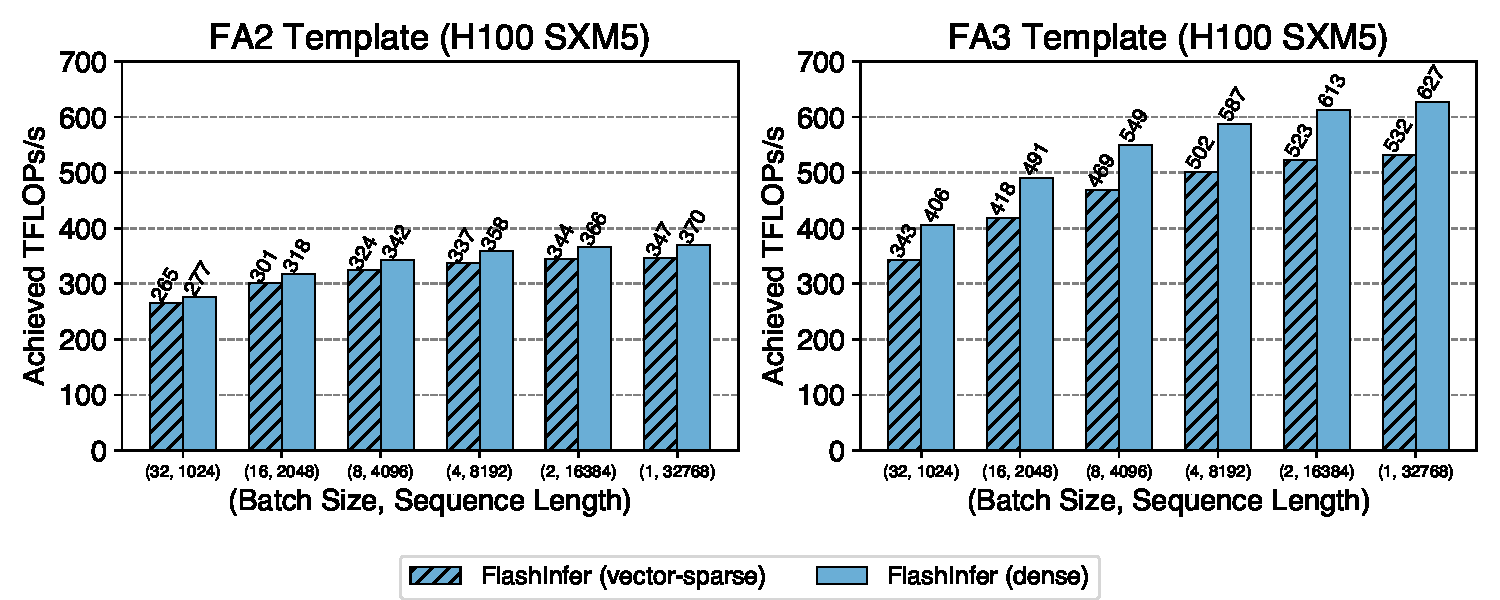
\includegraphics[width=0.4\textwidth]{figures/prefill-sparse-dense.pdf}
    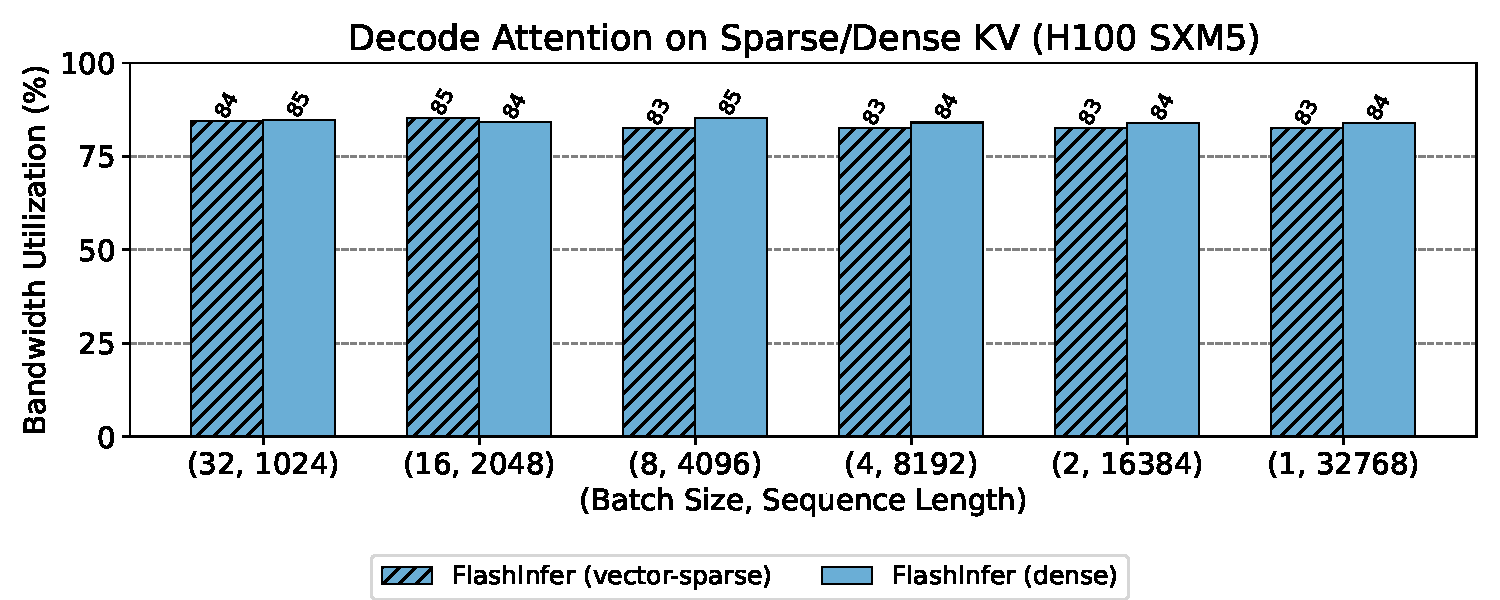
\includegraphics[width=0.4\textwidth]{figures/decode-sparse-dense.pdf}
    \caption{\textbf{上：} 在 FA2/FA3 模板下，使用稠密/稀疏 KV-Cache 的（因果）prefill 注意力内核达到的 TFLOPs/s。
    \textbf{下：} 使用稠密/稀疏 KV-Cache 的 decode 注意力内核带宽利用率。
    稀疏 KV-Cache 采用 page size 为 1（向量稀疏）的 PageAttention。横轴为不同 batch size 与序列长度。}
    \label{fig:sparse-dense}
\end{figure}

图~\ref{fig:sparse-dense} 对比了稀疏与稠密（连续）KV-Cache 在 prefill 与 decode 内核下的吞吐。
prefill 内核使用 \textit{causal} 注意力场景，这是 LLM 服务中的常见设置。对于连续 KV-Cache，我们使用变长 RaggedTensor prefill API\footnote{\url{https://docs.flashinfer.ai/api/prefill.html\#flashinfer.prefill.BatchPrefillWithRaggedKVCacheWrapper}}；对于稀疏 KV-Cache，我们使用 PagedKVCache prefill API\footnote{\url{https://docs.flashinfer.ai/api/prefill.html\#flashinfer.prefill.BatchPrefillWithPagedKVCacheWrapper}}。

query 头数与 KV 头数固定为 32，head dimension 设为 128。我们变化 batch size 与序列长度测量吞吐。decode 内核中，稀疏与稠密 KV-Cache 的性能差距可以忽略（在 $1\%$ 以内）；prefill 内核中，约有 $10\%$ 的差距。

需要注意，FA3 模板中的稠密注意力在 key/value 加载时使用 TMA（Tensor Memory Access）指令，而稀疏 gather 无法使用该机制，因为 Hopper 的 TMA 仅支持定步长访问，而稀疏 gather 需要任意行索引。因此，FA3 稀疏 gather 需回退到 Ampere 风格异步拷贝与手动指针运算，这会增加寄存器消耗，并需减小 KV tile 大小以避免寄存器溢出，导致性能差距略大。相比之下，在 FA2 模板中（稀疏与稠密都使用 Ampere 异步拷贝）差距更小，因为二者使用相同 tile 大小。

当块稀疏矩阵的列块大小较大（例如 128 及以上）时，稀疏 gather 可使用 TMA，因为每条 TMA 指令都可在单个固定步长块内工作。我们将该优化留作未来工作。不过，提高列块大小会降低块稀疏格式灵活性，不一定适用于所有场景。

\section{后端选择}
\label{sec:backend-choice}

在 NVIDIA GPU 上，我们选择在 CUDA/CUTLASS~\cite{cutlass} 之上构建 \sys，而非 Triton~\cite{triton}，主要原因如下：
\begin{enumerate}
    \item \textbf{更完整的 NVIDIA 新特性支持。} CUTLASS 支持 warp-specialization~\cite{warp-specialization}、TMA~\cite{hopper-tma} 等专用 GPU 能力，而这些能力在 Triton 中当前仍处于实验阶段或尚未支持。
    \item \textbf{更细粒度的内核优化能力。} Triton 提供 tile 级抽象，而 CUDA/CUTLASS 可进一步细化到线程级寄存器控制。这样的灵活性使我们更容易将低层优化（如 PTX intrinsic）直接并入 JIT 模板，这在 Triton 中更困难。
\end{enumerate}

我们的负载均衡调度器设计（第~\ref{sec:load-balanced-scheduling} 节）在很大程度上与后端无关，因此未来 \sys 可以集成 Triton，也可迁移到其他硬件平台。

\section{内存管理}
\label{sec:memory-mgmt}

\sys 管理一块页锁定（pinned）主机缓冲区和一块设备 workspace 缓冲区，用于存储调度器元数据与 split-k 部分输出。我们将设备 workspace 划分为多个 \emph{section}，每个 section 对应一组调度元数据数组或 split-k 部分输出数组。每次调度器 \lstinline{plan} 调用时，我们先在 pinned host buffer 上生成调度元数据，再通过 \lstinline{cudaMemcpyAsync} 异步拷贝到设备 workspace 的对应 section。

\subsection{兼容 CUDAGraph 的 Workspace 布局}
\label{sec:cudagraph-compatible-layout}

一旦内核被 CUDA Graph 捕获，其参数（指针与标量）会固定，因此设备 workspace 各 section 的地址在整个图生命周期内必须保持稳定。为此，我们按上界估计为每个 section 分配其最大容量（覆盖调度元数据与部分输出）。

\subsection{Split-K 的直写优化}
\label{sec:writethrough-optimizations}

在 \sys 的负载均衡调度器中（第~\ref{sec:load-balanced-scheduling} 节），仅 KV 长度较大的请求会进行 KV 切分。KV 较短请求无需切分，因此没有部分输出归约步骤。为节省计算与 workspace 内存，这些短请求可将部分输出直接写入最终输出缓冲区（绕过设备 workspace）。该策略同时降低了 workspace 需求与 contraction 内核计算负载。

\subsection{Workspace 缓冲区大小估计}
\label{sec:workspace-buffer-size}

workspace 大小主要由两部分决定：
(1) 调度元数据所需空间；
(2) split-k 部分输出所需空间。

\paragraph{调度元数据。} 每个元数据 section 的最大大小由“最大并发请求数”与“最大累计请求长度”决定。用户需在调度器首次计划阶段提供这些上界。

\paragraph{部分输出。} 部分输出大小取决于问题维度（头数与 head dimension）以及每次内核启动的 CTA 数。按我们的负载均衡算法~\ref{sec:load-balanced-scheduling}，只有“长请求”（即 KV 长度超过总 KV 长度除以 CTA 数）才会被切分。根据第~\ref{sec:writethrough-optimizations} 节的直写优化，只有这些切分请求会在 workspace 中产生输出。由于切分数不超过 CTA 总数，且每次切分最多产生两个需合并的 tile，因此部分输出最多为 \(2 \times \#\text{CTA}\)。每个 tile 产生大小为 \(T_q \cdot H_{qo} \cdot (D+1)\) 的部分输出，其中 \(T_q\) 是 query tile 大小，\(H_{qo}\) 为头数，\(D+1\) 为 head dimension 加 LSE 维度。因此部分输出总大小上界为：
\[
  2\,\#\text{CTA} \times T_q \times H_{qo} \times (D + 1).
\]
默认情况下，CTA 总数设为 $k \times \#\text{SM}$，其中 $\#\text{SM}$ 为 GPU 上流式多处理器数量，$k$ 选择为可最大化 CTA 级占用率。对于寄存器占用高的 Tensor Core 微内核，Ampere 上 $k$ 通常不超过 2；Hopper 上通常为 1（每个 SM 一个 CTA，也称持久化内核）。

\section{注意力与其他算子的重叠执行}
\label{sec:overlap-attention}

Nanoflow~\cite{zhu2024nanoflow} 在不同 CUDA stream 中重叠执行 GEMM、注意力与跨设备通信，并为每类操作分配固定 SM 数量。在 \sys 中，用户可通过 plan 函数传入该 SM 数，\sys 的负载均衡调度器会据此分配 tile。

\section{FP8--FP16 混合精度注意力}
\label{sec:mixed-precision}

近期 LLM 常采用 \texttt{fp8} KV-Cache 来降低内存带宽与存储成本~\cite{micikevicius2022fp8}。在 \sys 中，我们实现了\emph{混合精度}注意力内核：query 与 output 保持 \texttt{fp16}，KV-Cache 存储为 \texttt{fp8}。我们利用 \citet{gupta2024mixed} 提出的快速数值数组转换器与 fragment shuffler 来加速反量化并高效处理位宽不匹配。该设计可在不显著损失数值精度的情况下，降低内存占用并提升带宽利用。


\section{额外评估}
\label{sec:additional-evaluation}

本节给出更多实验结果，以进一步验证 \sys 在不同实验条件下的性能、可扩展性与鲁棒性。

\subsection{与 FlexAttention 的比较}

我们在 NVIDIA H100 80GB SXM 上使用 AttentionGym~\cite{AttentionGym} 基准比较 \sys 与 FlexAttention~\cite{he2024flexattention} 在不同注意力变体下的性能。
评测配置为 batch size $16$、头数 $16$、head dim $128$，CUDA 版本与 Triton 版本分别固定为 12.4 与 3.2。
表 \ref{table:flexattention-causal-attn} 至 \ref{table:flexattention-sliding-window} 给出 \sys 与 FlexAttention 的 TFLOPS/s（越高越好）。
在四类场景和多种序列长度下，\sys 均稳定优于 FlexAttention，且在长序列下优势更明显。
性能提升主要来自对 Hopper 架构高级特性的利用（如 warp specialization 与 TMA），以及 CUTLASS 相比 Triton 更细粒度的资源控制（寄存器级而非 tile 级）。随着 Triton 对这些特性的完整支持，差距预计会缩小。

\begin{table}[h]
\centering
\caption{因果注意力}
\label{table:flexattention-causal-attn}
\begin{tabular}{lrr}
\toprule
序列长度 & FlexAttention & \sys \\
\midrule
512   & 209.11 & \textbf{250.454} \\
1024  & 294.53 & \textbf{406.554} \\
2048  & 376.90 & \textbf{487.236} \\
4096  & 421.00 & \textbf{548.388} \\
8192  & 441.26 & \textbf{587.903} \\
16384 & 453.57 & \textbf{612.259} \\
\bottomrule
\end{tabular}
\end{table}

\begin{table}[ht]
\centering
\vspace{-10pt}
\caption{带 Logits SoftCap 的注意力}
\label{table:flexattention-logits-softcap}
\begin{tabular}{lrr}
\toprule
序列长度 & FlexAttention & \sys \\
\midrule
512   & 241.51 & \textbf{336.487} \\
1024  & 327.50 & \textbf{409.534} \\
2048  & 379.57 & \textbf{468.769} \\
4096  & 403.39 & \textbf{489.667} \\
8192  & 407.82 & \textbf{515.573} \\
16384 & 409.89 & \textbf{520.935} \\
\bottomrule
\end{tabular}
\end{table}

\begin{table}[ht]
\centering
\caption{ALiBi 偏置~\cite{press2022alibi}}
\label{table:flexattention-alibi}
\begin{tabular}{lrr}
\toprule
序列长度 & FlexAttention & \sys \\
\midrule
512   & 253.22 & \textbf{403.899} \\
1024  & 344.70 & \textbf{500.220} \\
2048  & 406.14 & \textbf{535.498} \\
4096  & 426.13 & \textbf{561.324} \\
8192  & 436.35 & \textbf{573.493} \\
16384 & 434.86 & \textbf{578.005} \\
\bottomrule
\end{tabular}
\end{table}

\begin{table}[ht]
\centering
\vspace{-3pt}
\caption{滑动窗口（窗口大小 = $1024$）}
\label{table:flexattention-sliding-window}
\begin{tabular}{lrr}
\toprule
序列长度 & FlexAttention & \sys \\
\midrule
512   & 206.51 & \textbf{236.363} \\
1024  & 292.25 & \textbf{374.108} \\
2048  & 350.91 & \textbf{381.464} \\
4096  & 368.45 & \textbf{384.998} \\
8192  & 373.25 & \textbf{384.514} \\
16384 & 367.91 & \textbf{380.506} \\
\bottomrule
\end{tabular}
\end{table}


\subsection{共享前缀注意力内核评估}

我们在后缀长度为 $128$ 下评估共享前缀注意力内核。
表~\ref{table:eval-shared-prefix-attn} 给出了不同共享前缀长度、不同场景和不同 batch size 下的内核时延（单位：微秒，us），其中 “composable” 表示可组合格式，“single” 表示单格式。
可组合格式在长前缀（如 32k）和大 batch（如 $64$）下收益明显。
不过这些内核级提升不总能线性转化为端到端收益，因为真实场景中的共享前缀通常更短。

\begin{table}[hbt]
\small
\centering
\caption{共享前缀注意力内核时延}
\label{table:eval-shared-prefix-attn}
\begin{tabular}{lr@{}r@{}r@{}r@{}}
\toprule
\makecell{共享\\前缀\\长度} & \makecell{Composable\\(BS=16)} & \makecell{Single\\(BS=16)} & \makecell{Composable\\(BS=64)} & \makecell{Single\\(BS=64)} \\
\midrule
1024   & \textbf{45.17}  & 46.52  & 87.86   & 130.49 \\
8192   & \textbf{88.67}  & 226.57 & 125.76  & 931.75 \\
32768  & \textbf{217.42} & 945.67 & 254.54  & 4090   \\
\bottomrule
\end{tabular}
\end{table}

\subsection{变长序列与负载均衡调度消融}

我们对负载均衡调度器（第~\ref{sec:load-balanced-scheduling} 节）的效果进行消融。
表~\ref{table:eval-ablation-itl} 与~\ref{table:eval-ablation-ttft} 展示了 Llama 3.1-8B-Instruct 在 NVIDIA H100 SXM5 上、SGLang~\cite{zheng2023sglang} + \sys（启用/禁用负载均衡调度）下的结果。
我们评估三类数据集上的 ITL（ms）与 TTFT（ms）：ShareGPT、输入长度采样自 $U(512,2048)$ 且输出固定为 $256$ 的变长集、输入长度采样自 $U(4096,16384)$ 且输出固定为 $256$ 的变长集。表中 “RR” 表示请求率。

\begin{table}[hbt]
\small
\centering
\vspace{-5pt}
\caption{负载均衡调度消融（ITL）}
\label{table:eval-ablation-itl}
\begin{tabular}{@{}lrrr@{}}
\toprule
场景 & \makecell{启用\\负载\\均衡} & \makecell{禁用\\负载\\均衡} & Triton \\
\midrule
ShareGPT (RR=16) & \textbf{8.96} & 9.16 & 9.36 \\
$U(512, 2048)$ (RR=8)        & \textbf{8.21} & 8.42 & 8.49 \\
$U(4096, 16384)$ (RR=1)        & \textbf{8.63} & 13.89 & 11.08 \\
\bottomrule
\end{tabular}
\end{table}

\begin{table}[hbt]
\small
\centering
\caption{负载均衡调度消融（TTFT）}
\label{table:eval-ablation-ttft}
\begin{tabular}{@{}lrrr@{}}
\toprule
场景 & \makecell{启用\\负载\\均衡} & \makecell{禁用\\负载\\均衡} & Triton \\
\midrule
ShareGPT (RR=16) & \textbf{39.05} & 39.42 & 52.92 \\
 $U(512, 2048)$ (RR=8)        & \textbf{66.78} & 67.38 & 68.48 \\
 $U(4096, 16384)$ (RR=1)        & \textbf{411.02} & 421.60 & 566.30 \\
\bottomrule
\end{tabular}
\end{table}

\subsection{vLLM 集成评估}

我们在固定请求率 $16$ 下比较 vLLM 的 \sys 后端与默认后端，并在表~\ref{table:eval-vllm-integration} 报告吞吐（tokens/s）、ITL（ms）与 TTFT（ms）。
在 fp8 KV-cache 下，\sys 的 ITL 可降低约 13\%；但在 bf16 下，vLLM 集成中的主机侧 Python 开销（如数组操作）会带来轻微回退。未来我们将通过 C++ 化并将调度器下沉到设备端来优化。

\begin{table}[hbt]
\centering
\caption{vLLM 集成评估}
\label{table:eval-vllm-integration}
\begin{tabular}{@{}l@{}rrr@{}}
\toprule
后端         & 吞吐 & \makecell{中位\\ITL} & \makecell{中位\\TTFT} \\
\midrule
Default (bf16)  & 6062.89    & 10.42      & 35.85      \\
\sys (bf16)    & 6065.41    & 10.63      & 36.60      \\
Default (e4m3)  & 6015.86    & 12.56      & 39.74      \\
\sys (e4m3)    & 6020.32    & 10.92      & 37.93      \\
\bottomrule
\end{tabular}
\end{table}

\subsection{细粒度块稀疏评估}

\sys 支持细粒度块稀疏矩阵，这对多种 KV-Cache 剪枝算法很有价值。
我们在 Quest~\cite{tang2024quest} 上测量内核性能。Quest 是一种 SOTA 长上下文建模算法，KV-Cache 采用细粒度稀疏。
我们在 NVIDIA H100 SXM5 上对 Quest 的批量解码注意力内核进行比较，评估 \sys、PyTorch SDPA 与 FlexAttention，配置为（block size 16，num\_qo\_heads $32$，num\_kv\_heads $32$，head\_dim $128$）。
所有时延单位均为微秒（us）。

如表~\ref{table:eval-sparsity-flashinfer} 至~\ref{table:eval-sparsity-flexattention} 所示，\sys 具有显著性能优势，在长序列下最高可达 20x 加速。
目前 FlexAttention 依赖大块大小模板，而 \sys 采用 sparse-row gather 策略，在小块大小下也能利用稠密 Tensor Core。该设计天然支持细粒度 KV-cache 剪枝。

\begin{table}[hbt]
\small
\centering
\caption{\sys 细粒度稀疏时延（us）}
\label{table:eval-sparsity-flashinfer}
\begin{tabular}{@{}lrrrr@{}}
\toprule
\multicolumn{1}{c}{} & \multicolumn{4}{c}{page\_budget} \\
\cmidrule(l){2-5}
seq\_len & 64 & 128 & 256 & 512 \\
\midrule
4096  & 20.299 & 30.361 & 44.383 & 44.430 \\
8192  & 22.273 & 28.603 & 44.928 & 68.194 \\
16384 & 20.485 & 28.678 & 44.677 & 68.700 \\
32768 & 22.371 & 28.700 & 44.988 & 68.478 \\
\bottomrule
\end{tabular}
\end{table}

\begin{table}[hbt]
\small
\centering
\caption{PyTorch SDPA 细粒度稀疏时延（us）}
\label{table:eval-sparsity-torch}
\begin{tabular}{@{}lrrrr@{}}
\toprule
\multicolumn{1}{c}{} & \multicolumn{4}{c}{page\_budget} \\
\cmidrule(l){2-5}
seq\_len & 64 & 128 & 256 & 512 \\
\midrule
4096  & 287.684 & 288.904 & 287.715 & 287.807 \\
8192  & 474.631 & 474.508 & 474.683 & 473.070 \\
16384 & 857.319 & 857.570 & 857.094 & 857.728 \\
32768 & 1711.955 & 1711.621 & 1713.093 & 1711.709 \\
\bottomrule
\end{tabular}
\end{table}

\begin{table}[hbt]
\small
\centering
\caption{FlexAttention 细粒度稀疏时延（us）}
\label{table:eval-sparsity-flexattention}
\begin{tabular}{@{}lrrrr@{}}
\toprule
\multicolumn{1}{c}{} & \multicolumn{4}{c}{page\_budget} \\
\cmidrule(l){2-5}
seq\_len & 64 & 128 & 256 & 512 \\
\midrule
4096  & 1100.349 & 1097.356 & 1073.753 & 1071.797 \\
8192  & 1092.695 & 1099.100 & 1078.081 & 1074.886 \\
16384 & 1109.817 & 1101.535 & 1077.639 & 1076.859 \\
32768 & 1169.109 & 1187.395 & 1176.332 & 1174.502 \\
\bottomrule
\end{tabular}
\end{table}
